\documentclass[10pt,a4paper]{article}
\usepackage[utf8]{inputenc}
\usepackage{amsmath}
\usepackage{amsfonts}
\usepackage{amssymb}
%\usepackage{apacite}
\usepackage{parskip}
\usepackage{url}
\usepackage{graphicx}

\newcommand{\note}[1]{\marginpar{\textit{#1}}}
\newcommand{\todo}[1]{\marginpar{\textbf{TODO:} #1}}
\newcommand{\TODO}[1]{\textbf{TODO: #1}}

\author{Benedikt Kristinsson}
\title{Cryptographically Secure Pseudo-random Generation on the Arduino}
\date{Working draft / Test results}

\begin{document}

\maketitle

\section{Introduction}

Generating randum number is something that might seem simple at first glance, but computers are deterministic in their nature and can't thus generate random numbers. Typically Random Number Generators (RNG) observe some physical phenomenon that has been shown to either be chaotic or random. Random numbers are very usable in cryptogrpahy since almost all cryptographic protocols and key schemas rely on the assumption that that attacker does not know the key. 

\section{Observerations}

Both the operating temperature and the size/volume of the space that the Arduino sits in while polling seems to affect the fluctuations of the \texttt{readAnalog} method. The larger the space --- the smaller the fluctuations (the fluctions are the inverse of the volume). Lower temperatures also cause more fluctuations.


\subsection{Samples}

 Figures 1 to 5 show samples of 50 000 values taken under different conditions. The polling interval was set to 0.01 seconds in all cases. 

\subsubsection{Room temperature, different spaces}

At room temperatures we see that the \texttt{analogRead} method behaves similarily, but seemt to be affected y the space around it and temperature changes. 

\begin{figure}[H!]
  \caption{50000 samples at room temperatures}
  \centering
  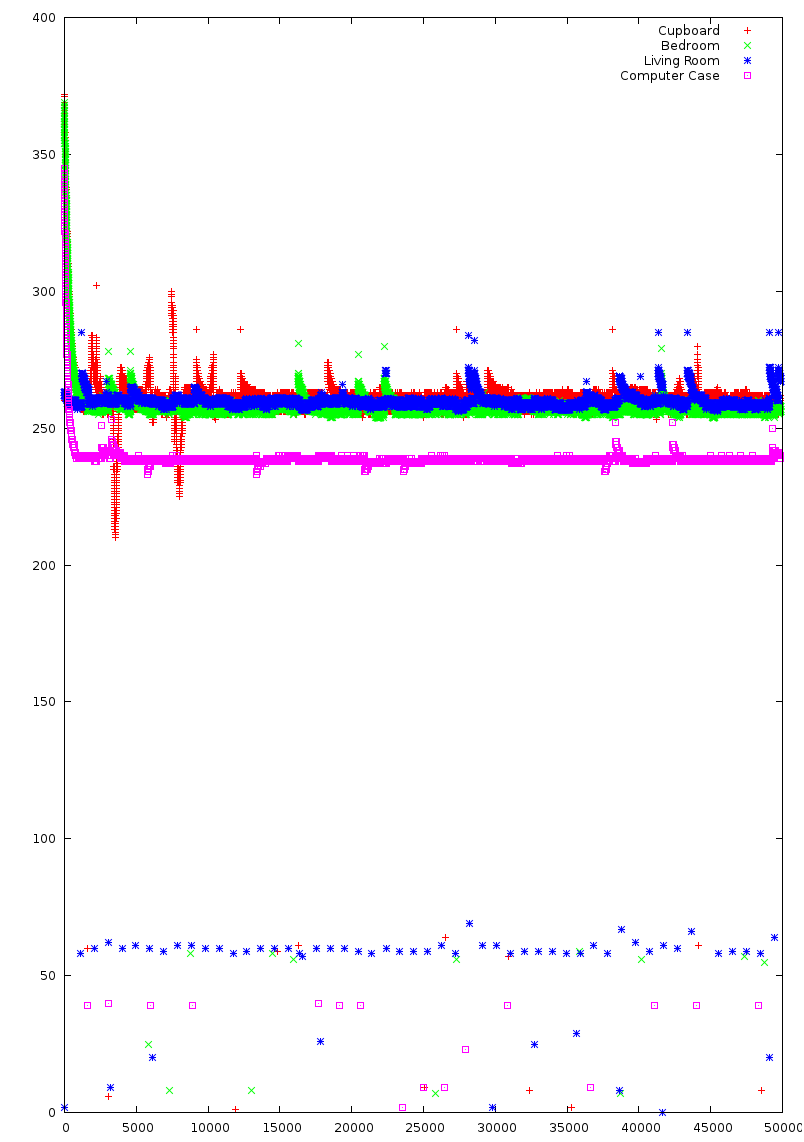
\includegraphics[width=0.5\textwidth]{img/RoomTempOverlay.png}
\end{figure}


\begin{figure}[H!]
  \caption{Collected in a $50m^2$ area}
  \centering
  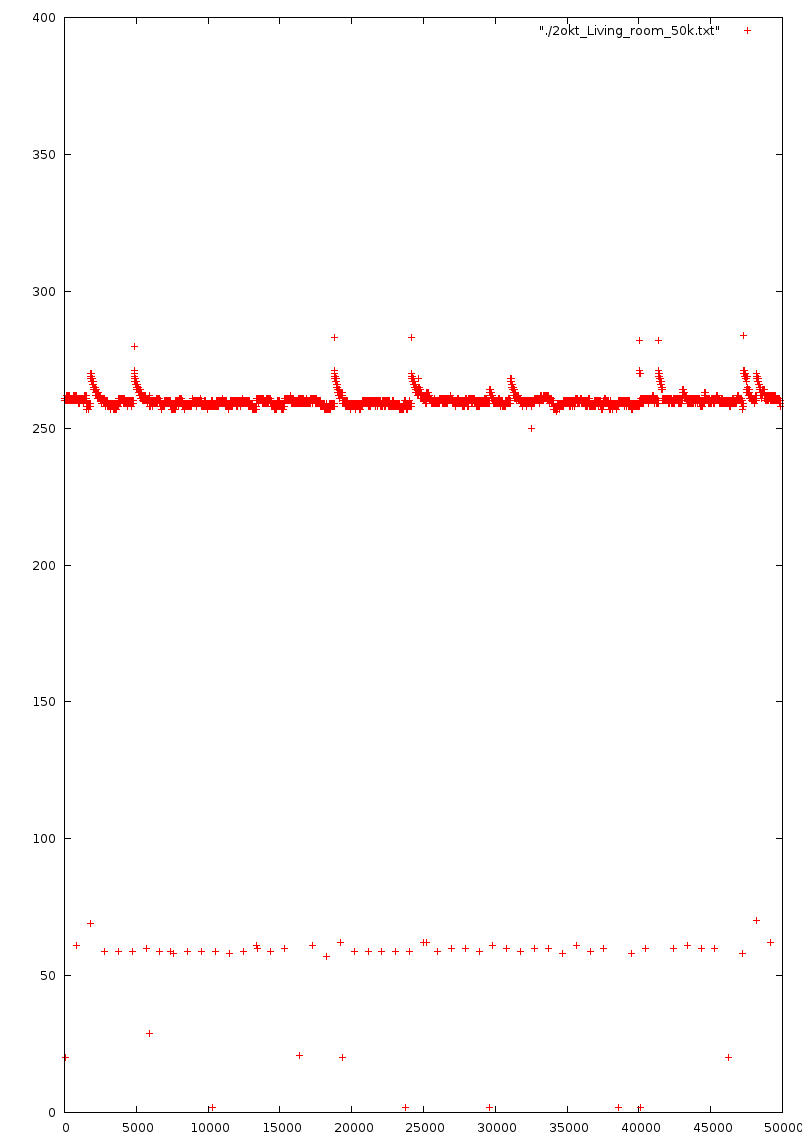
\includegraphics[width=0.5\textwidth]{img/LivingRoom50kFull.png}
\end{figure}

\begin{figure}[H!]
  \caption{Collected in a $12m^2$ area}
  \centering
  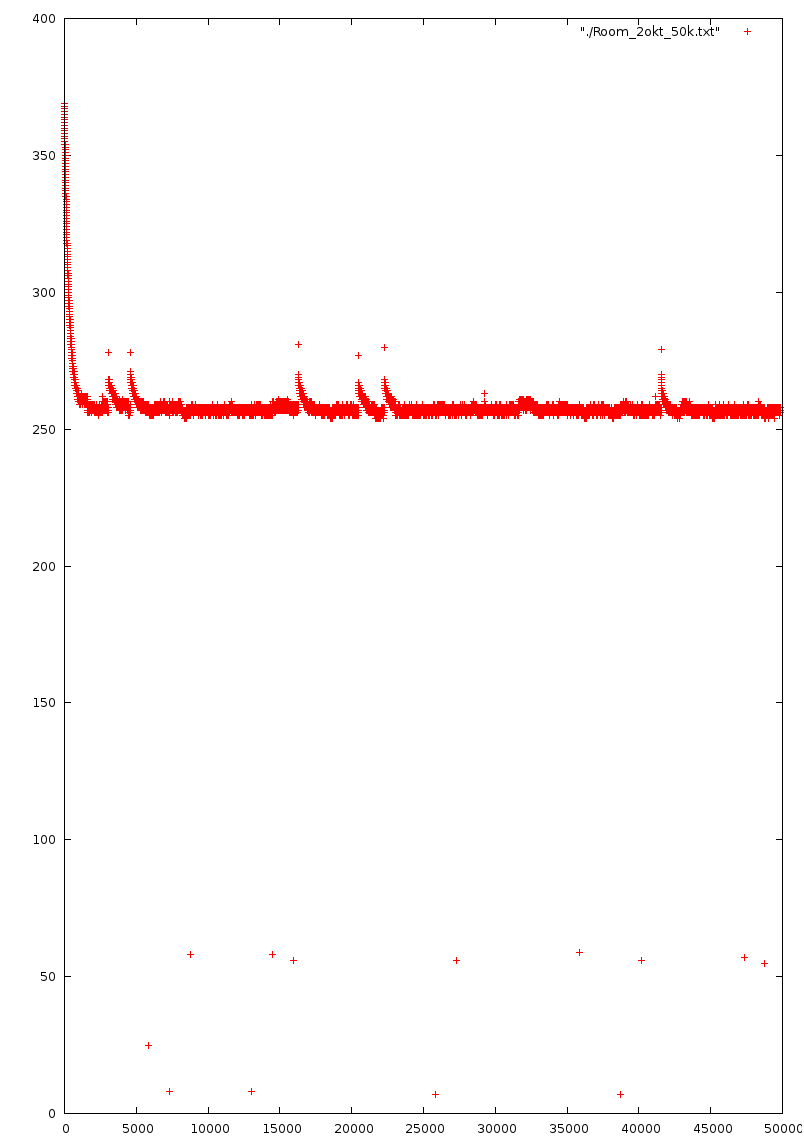
\includegraphics[width=0.5\textwidth]{img/Bedroom50kFull.png}
\end{figure}

\begin{figure}[H!]
  \caption{Collected in a small wooden cupboard}
  \centering
  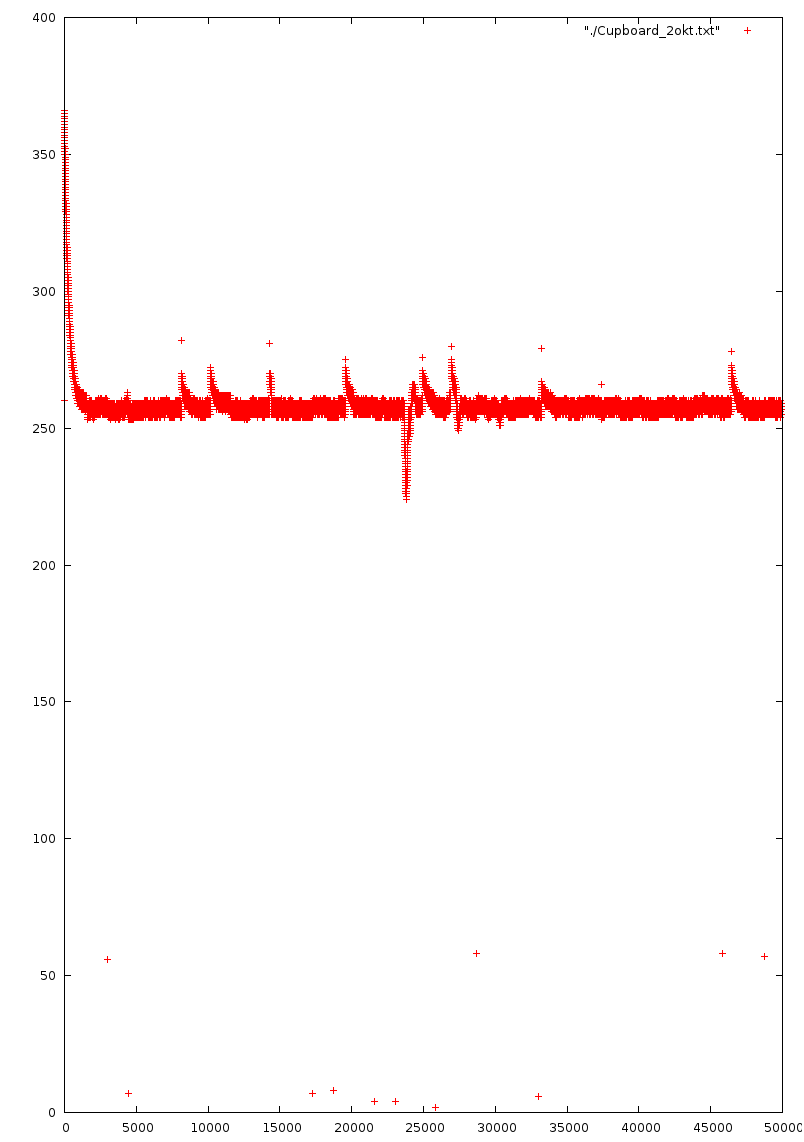
\includegraphics[width=0.5\textwidth]{img/Cupboard50kFull.png}
\end{figure}

\begin{figure}[H!]
  \caption{Collected inside a Cheiftech Dragon computer case, temperature above room temp}
  \centering
  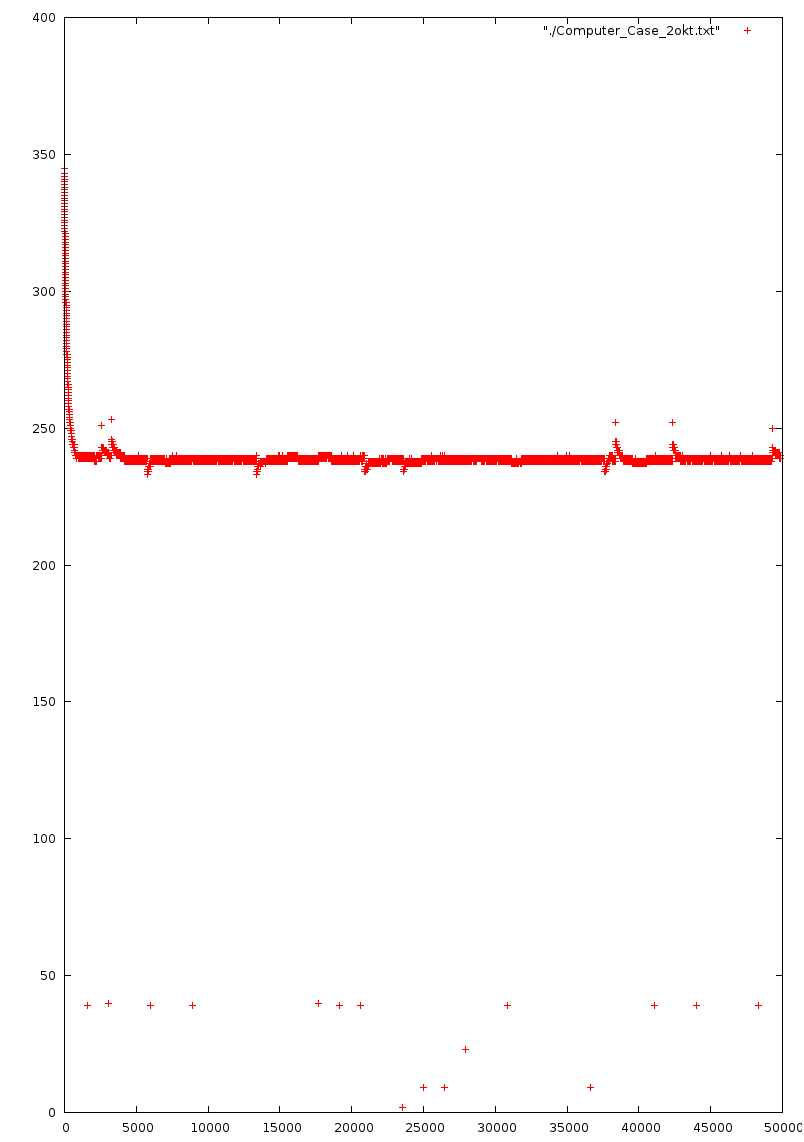
\includegraphics[width=0.5\textwidth]{img/ComputerCase50.png}
\end{figure}


\subsubsection{Extreme temperatures}

The oeprating temperatures for the ATMega 328 CPU on the Arudino is -40C to +85C \cite{atmegads} (Arudino themselves have not published operating temperatures themselves) and these temperatures are within that range\footnote{I haven't measured freezer or heating element yet, but I have a hunch}. The Arudino does not operate reliable inside the freezer so that sample consists only of 10 000 values. Note that these graps are showing an $y$-axis range of $0..400$ and (very) few singelton values lie above 400. 

\begin{figure}[H!]
  \caption{Collected inside a fridge at temperature 1C} %% TEMP
  \centering
  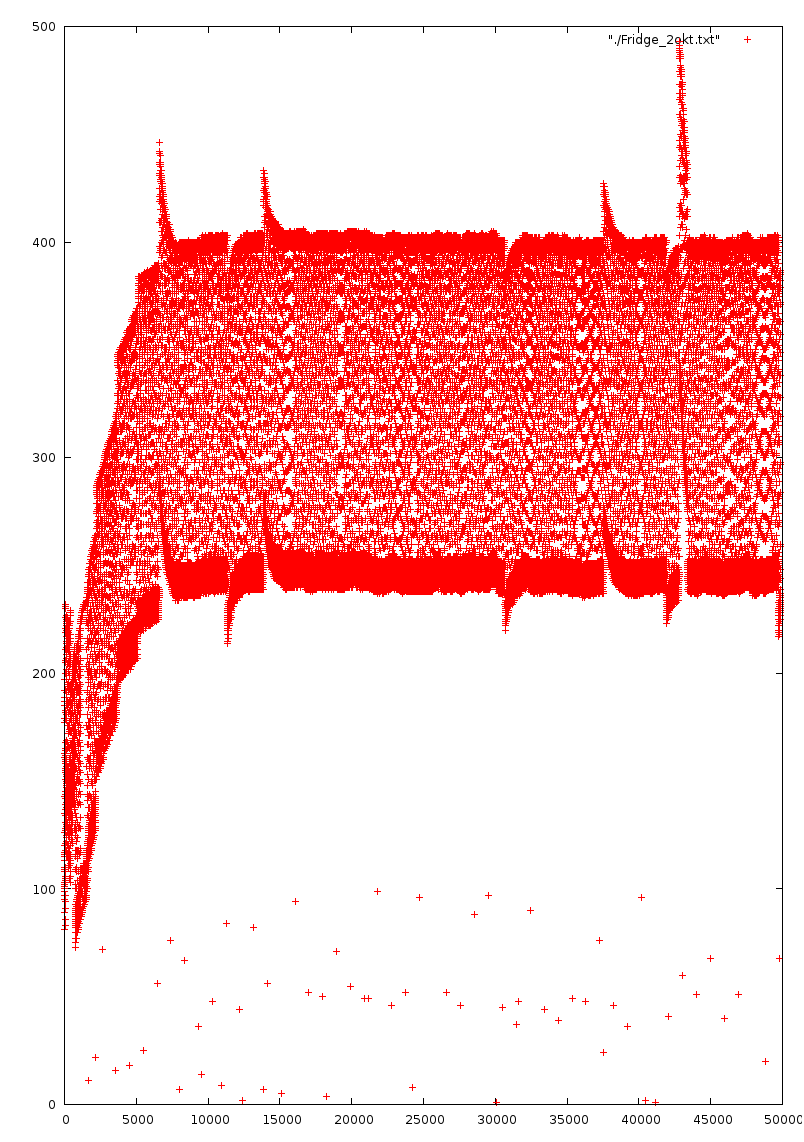
\includegraphics[width=0.5\textwidth]{img/Fridge50k.png}
\end{figure}

\begin{figure}[H!]
  \caption{10000 values collected inside a freezer at temperature ??C} %% TEMP
  \centering
  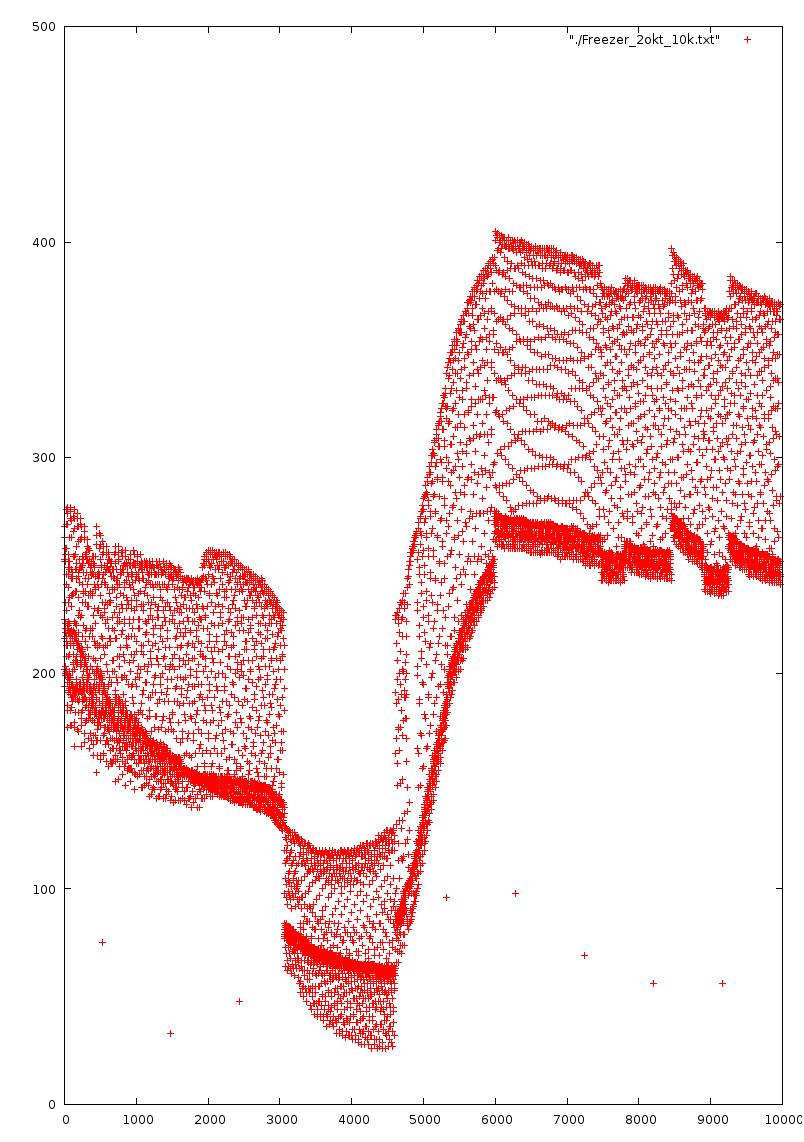
\includegraphics[width=0.5\textwidth]{img/Freezer10k.png}
\end{figure}

\begin{figure}[H!]
  \caption{Collected on a heating element at temperature ??C} %% TEMP
  \centering
  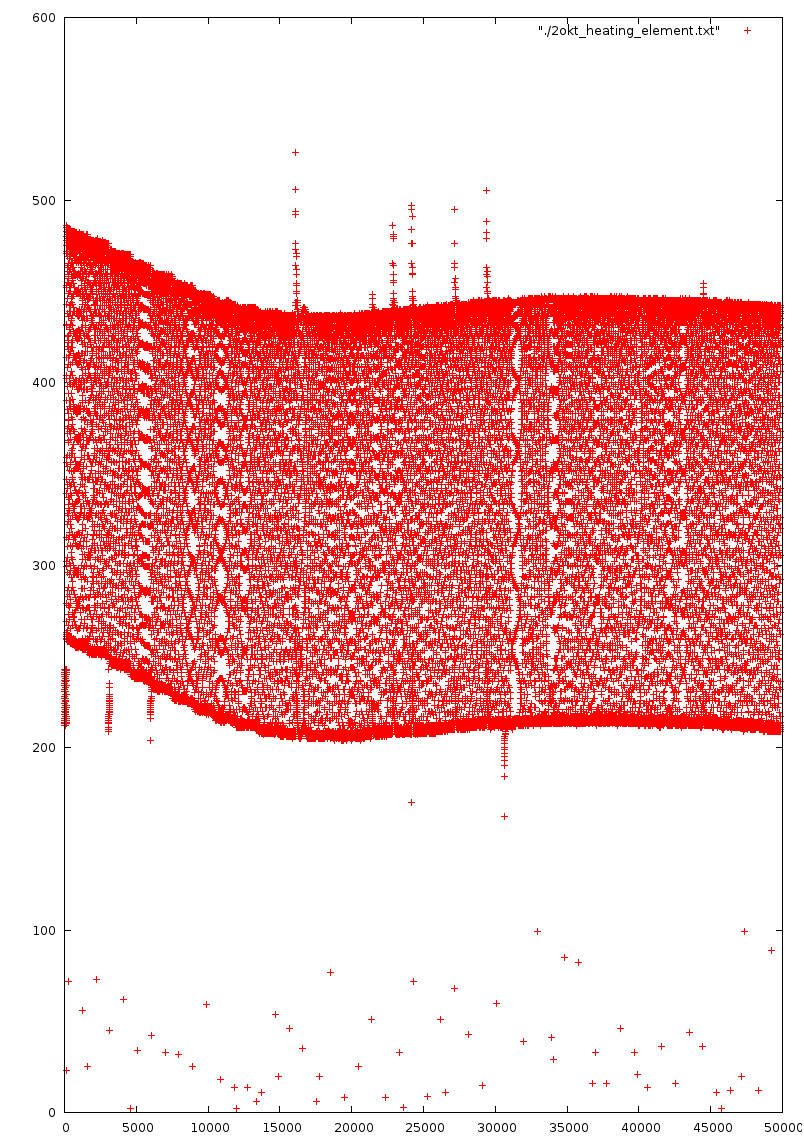
\includegraphics[width=0.5\textwidth]{img/Heating50k.png}
\end{figure}


\section{Placeholder}

\cite{anthes2011} \cite{airturb} \cite{nist} \cite{intel} \cite{atmegads} \cite{menezes1996} \cite{schneier1996} \cite{maurer1998}

\bibliography{ardrand}{}
\bibliographystyle{plain}

\end{document}